\specialsection{Обзор литературы и предметной области}

Тема применения нейронных сетей в контексте решения формально-логических задач развита не особо сильно, поскольку дискретные задачи со строгими ограничениями тяжело даются сетям с известными на данный момент архитектурами. Тем не менее, известны многочисленные попытки использовать нейросети в качестве помощника для алгоритма, решающего ту или иную задачу. Про несколько таких подходов, имеющих отношение к проверке выполнимости и поиску решения для SMT-формул, я расскажу далее. Но перед этим я детально опишу устройство и архитектуру графовых нейронных сетей, поскольку на использовании данной архитектуры в значительной части основана моя работа.

\specialsubsection{Устройство GNN} \label{gnn-architecture}

Графовые нейронные сети\footnote{Далее по тексту будем называть их GNN (англ. \textit{Graph Neural Networks}).}, наряду со свёрточными, рекуррентными и т. д., являются одним из способов решать задачу машинного обучения, учитывая специфику данных. Так как графы отображают взаимоотношения между объектами некоторого множества, то и процесс построения модели, в данном случае, учитывает локальность и связи между произвольными объектами из предметной области.

Впервые архитектура GNN в общем виде была описана ещё в 2009 году в статье \cite{gnn-intro-paper}, однако широкую известность получила только в 2017 году после её применения для предсказания квантовых чисел в вычислительной органической химии \cite{gnn-quantum-chemistry-paper}. В основе вычислений лежит процесс \textit{передачи сообщений} между вершинами графа, который изображён\footnote{Подобное вычисление происходит для каждой вершины на каждой итерации процесса \textit{передачи сообщений}.} на рис.~\ref{message-passing-nn-architecture}: в каждой вершине хранится вектор-состояние (эмбеддинг\footnote{От англ. \textit{embedding} --- в машинном обучении так называют представление некоторого объекта в многомерном векторном пространстве.}), и на каждом шаге все вершины сначала рассылают свой текущий вектор всем своим непосредственным соседям, а потом агрегируют пришедшие от соседей векторы (\textit{сообщения}) и обновляют свой вектор-состояние с учётом этого; далее эти шаги повторяются несколько раз, после чего полученные таким образом векторы-состояния используются для построения представления графа и дальнейшего решения задачи.

\begin{figure}[ht]
\begin{center}
    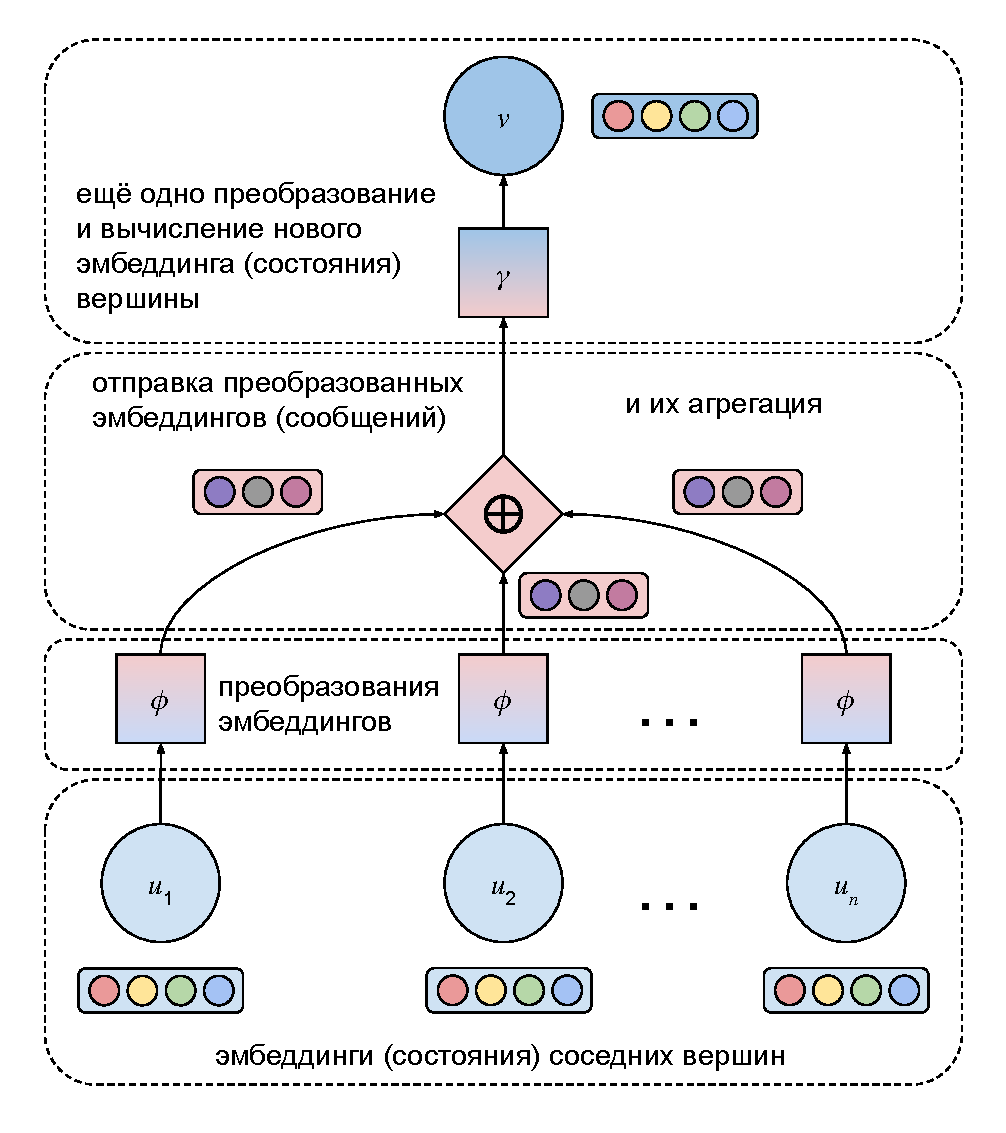
\includegraphics[scale=0.75]{./assets/message-passing-nn-architecture.pdf}
    \caption{\label{message-passing-nn-architecture} Схема обновления вектора-состояния вершины $v$ через векторы-сообщения от её соседей $u_1$, $u_2$, \ldots, $u_n$. Цвет (синий / красный) обозначает размерность. Более тёмный цвет вверху обозначает обновлённое состояние.}
\end{center}
\end{figure}

Согласно \cite{gnn-deep-learning-5g}, формально весь процесс устроен следующим образом:

\begin{itemize}
    \item у каждого ребра $e$ есть набор параметров $s_e \in \mathbb{R}^m$;
    \item в начале вычислений в каждой вершине $v$ содержится содержится вектор (состояние) $x_v^{(0)} \in \mathbb{R}^n$ с некоторой информацией;
    \item производится несколько итераций \textit{передачи сообщений}, на $t$-й из них производится обновление векторов в вершинах по правилу, которое описывается формулой~(\ref{gnn-state-update-rule});
    \item после всех итераций предполагается, что вычисленные векторы (состояния) образуют некоторое представление вершины / графа, поэтому их можно использовать в качестве параметров\footnote{Будем также называть их признаками или фичами (от англ. \textit{feature}).} вершины / графа, подавая в какую-нибудь MLP\footnote{Многослойный перцептрон (от англ. \textit{Multi-Layer Perceptron}) --- последовательная комбинация из полносвязных линейных слоёв и нелинейных слоёв активации.}-сеть.
\end{itemize}

\begin{equation} \label{gnn-state-update-rule}
    x_v^{(t)} = \gamma^{(t)} \left(x_v^{(t - 1)}, \bigoplus_{u \in \mathcal{N}(v)} \phi^{(t)} \left(x_v^{(t - 1)}, x_u^{(t - 1)}, s_{e(u \, \to \, v)} \right) \right)
\end{equation}

Обозначения в формуле~(\ref{gnn-state-update-rule}):

\begin{itemize}
    \item $x_v^{(t)} \in \mathbb{R}^n$ --- описанные выше эмбеддинги вершин;
    \item $e(u \, \to \, v)$ --- ребро из вершины $u$ в вершину $v$, а $s_{e(u \, \to \, v)} \in \mathbb{R}^m$ --- его параметры;
    \item $\mathcal{N}(v)$ --- окрестность вершины $v$;
    \item $\phi^{(t)}: \mathbb{R}^n \times \mathbb{R}^n \times \mathbb{R}^m \to \mathbb{R}^k$ --- функция создания сообщения по состояниям вершин и параметрам ребра; может быть представлена аффинным преобразованием, композицией линейных слоёв и нелинейных активаций, какими-нибудь сложными LSTM\footnote{Долгая краткосрочная память (от англ. \textit{Long Short-Term Memory}) --- известная модификация рекуррентной нейронной сети.} или GRU\footnote{Управляемый рекуррентный блок (от англ. \textit{Gated Recurrent Unit}) --- ещё одна известная модификация рекуррентной нейронной сети.}-слоями или просто любым дифференцируемым преобразованием с обучаемыми или необучаемыми параметрами;
    \item $\bigoplus: \mathbb{R}^k \to \mathbb{R}^k$ --- функция агрегации, например: сумма, среднее или взвешенная сумма с учётом механизма внимания;
    \item $\gamma^{(t)}: \mathbb{R}^n \times \mathbb{R}^k \to \mathbb{R}^n$ --- функция обновления вектора-состояния (эмбеддинга) вершины; аналогична $\phi^{(t)}$.
\end{itemize}

В качестве примера построения сети по такой схеме можно рассмотреть Graph Convolutional Network \cite{gcn-conv-paper}, самую популярную GNN-архитектуру. В её случае мы имеем:

\begin{itemize}
    \item $\phi^{(t)} = W^T \cdot x_u^{(t - 1)}$;
    \item $\bigoplus = \sum \limits_{u \in \mathcal{N}(v) \cup \{v\}} \dfrac{1}{\sqrt{|\mathcal{N}(v)|} \cdot \sqrt{|\mathcal{N}(u)|}} \cdot \phi^{(t)} \left(x_v^{(t - 1)}, x_u^{(t - 1)}, s_{e(u \, \to \, v)} \right)$;
    \item $\gamma^{(t)} = \bigoplus \limits_{u \in \mathcal{N}(v)} \phi^{(t)} \left(x_v^{(t - 1)}, x_u^{(t - 1)}, s_{e(u \, \to \, v)} \right) + b$;
\end{itemize}

\noindent где матрица весов $W$ и вектор-сдвиг $b$ являются выучиваемыми параметрами. Итого получаем:

\begin{equation}
    x_v^{(t)} = \sum \limits_{u \in \mathcal{N}(v) \cup \{v\}} \dfrac{1}{\sqrt{|\mathcal{N}(v)|} \cdot \sqrt{|\mathcal{N}(u)|}} \cdot \left(W^T \cdot x_u^{(t - 1)} \right) + b
\end{equation}

В настоящий момент GNN широко применяются для решения задач вычислительной физики, химии и биологии, построения рекомендательных систем, прогнозирования трафика на дорогах, распознавания объектов, синтеза текстов и речи \cite{gnn-global-overview} \cite{gnn-deep-learning-5g}.

% todo: написать, что такая штука совмещает в себе CNN и RNN

\specialsubsection{FastSMT}

В статье \cite{fastsmt-paper} рассматривается идея повышения эффективности SMT-решателя за счёт оптимизации его работы на формулах, возникающих в задачах из фиксированной предметной области.

Решатель в процессе своей работы применяет к формуле большое количество разных семантически эквивалентных преобразований\footnote{В статьях и документациях их называют тактиками.}, чтобы привести её к некоторому удобному для себя виду, в котором он сможет либо достаточно быстро найти решение для формулы и доказать, что оно подходит (тем самым доказав, что формула является выполнимой), либо достаточно быстро доказать, что указанный в формуле набор ограничений невозможно выполнить, и формула является невыполнимой. Примеры тактик: замена переменной, нормализация границ неравенства, bit-blasting (представление переменной в виде набора пропозициональных значений), переписывание условного оператора через конъюнкцию импликаций и т. д.. Упомянутый ранее решатель Z3 \cite{z3-paper} поддерживает более ста подобных операций.

Цепочка преобразований, которые решатель производит над формулой, формируется согласно некоторой стратегии, которая учитывает самые разнообразные параметры (признаки) формулы: от её размера и количества свободных переменных до некоторого приближения абстрактно-синтаксического дерева формулы. Сама стратегия, в данном случае, больше всего похожа на решающее дерево, у которого в вершинах стоят ограничения на очередные параметры формулы, а в каждом листе находится тактика, которую стоит применить в случае, когда параметры соответствуют пути в этот лист.

Базовую стратегию, которая используется в решателе по-умолчанию, подбирают его создатели, причём они делают это так, чтобы его средняя скорость работы на произвольной формуле была как можно лучше. В результате, решатель работает более стабильно (т. е. реже уходит в экспоненциальный перебор возможных решений, когда на вход подают сложную формулу), но скорость нахождения ответа в более простых случаях из-за этого проседает.

В то же время, большинство популярных современных инструментов для решения SMT-формул поддерживают возможность использования специфических стратегий, которые можно построить, в том числе, самостоятельно. Помимо этого, есть некоторая интуиция, что если мы будем рассматривать только формулы из некоторой фиксированной практической задачи, то все эти формулы будут обладать некоторой спецификой, знание о которой сможет существенно помочь в проверке их выполнимости. На этой интуиции, а также на возможности использовать собственные стратегии при решении формул строится подход, описанный в рассматриваемой статье.

Главная идея состоит в следующем: набор признаков формулы можно рассматривать как состояние некоторой среды, применение очередной тактики можно рассматривать как некоторое действие, совершаемое в этой среде, а награду за последовательность применённых тактик можно определить как суммарное время работы решателя на заданной формуле с использованием этой последовательности (разумеется, взятое с минусом), либо какому-нибудь штрафному значению в случае, если решатель не справляется с формулой. Таким образом, задача поиска оптимальной стратегии применения различных тактик хорошо представляется в виде задачи обучения с подкреплением, где средой является произвольная формула из некоторой фиксированной задачи. Поэтому предлагается выучивать модель (политику), которая по текущему состоянию среды (формулы) будет выдавать оптимальную тактику и параметры для неё.

\begin{figure}[ht]
\begin{center}
    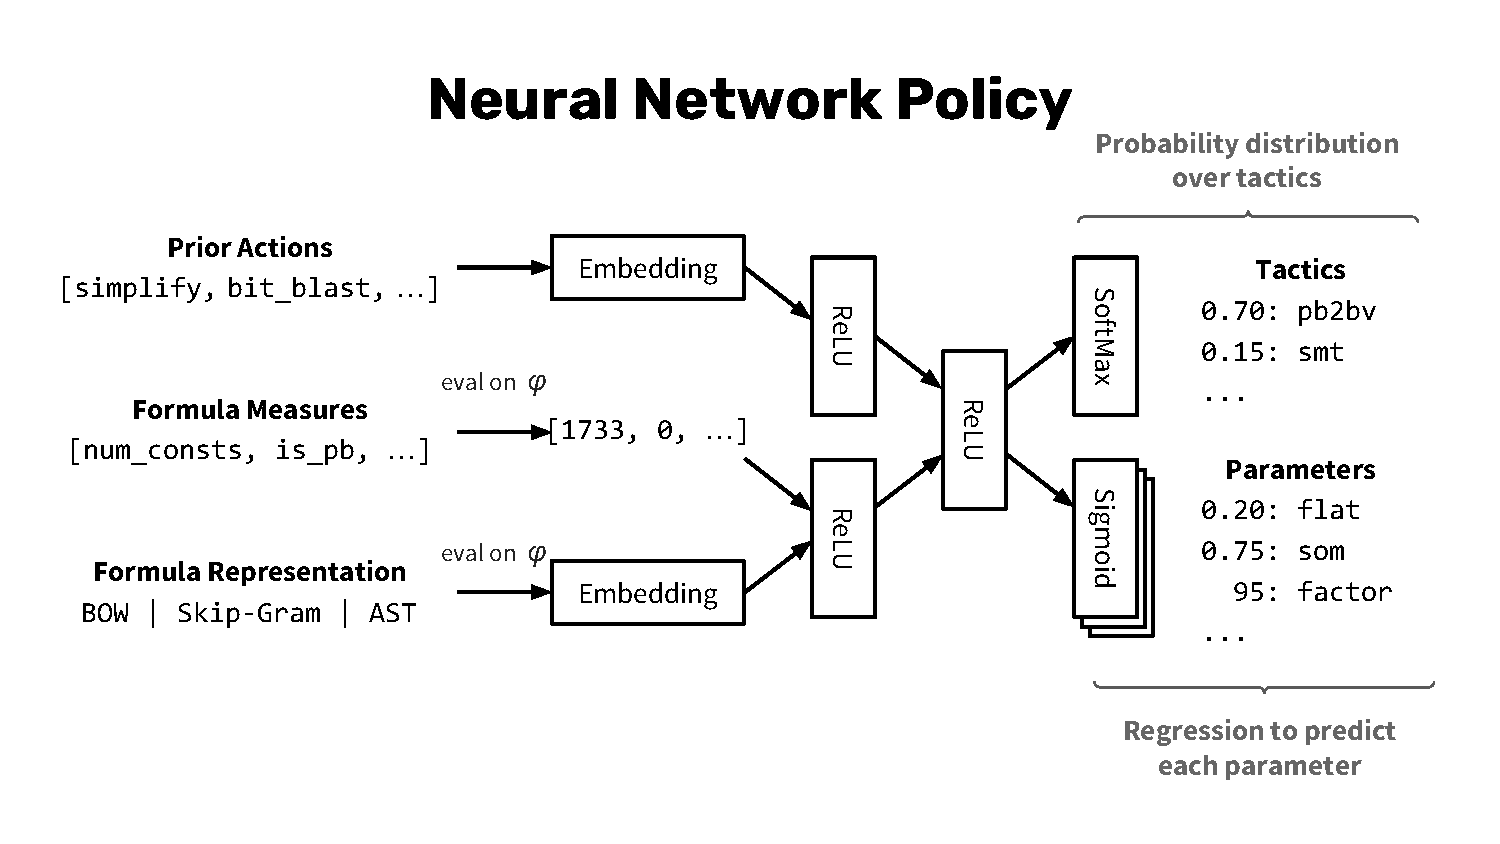
\includegraphics[scale=0.65]{./assets/fastsmt-nn-policy.pdf}
    \caption{\label{fastsmt-architecture} Архитектура модели. Картинка взята из статьи \cite{fastsmt-paper}.}
\end{center}
\end{figure}

Архитектура модели изображена на рис.~\ref{fastsmt-architecture}. На вход подаются признаки формулы (Formula Measures) и её синтаксическое представление, закодированное в виде bag-of-words или $n$-граммной модели (Formula Representation). Вдобавок к этому, для каждой тактики выучивается эмбеддинг, который хранит в себе семантическую информацию про неё. Эмбеддинги тактик, которые можно применить в данный момент, также подаются на вход модели (Prior Actions). На выходе у модели распределение на тактиках, которые стоит применить в данный момент, и значения параметров для них. Сразу отмечу, что, несмотря на то, что модель выдаёт распределение на всех доступных для применения в данный момент тактиках, за одно действие применяется только одна из них --- наиболее вероятная.

Построенная таким образом модель обучается на наборе формул взятом из некоторой задачи (в статье это были различные известные бенчмарки для решателей, на каждом из которых обучалась и оценивалась отдельная модель) с помощью метода, похожего на кросс-энтропийный метод. После этого с помощью техник семплирования строятся разнообразные статистики, отражающие выученную моделью политику, а уже на них обучается решающее дерево, выбирающее нужную тактику по текущей формуле, которое впоследствии превращается в стратегию, которую можно загрузить в SMT-решатель.

Авторы статьи заявляют, что, согласно проведённым экспериментам, предложенный подход позволяет успешно решать на 17\% больше формул при десятисекундном ограничении по времени, а также даёт прирост производительности вплоть до стократного ускорения на некоторых формулах (при этом, замедления при решении других формул не наблюдается). Тем не менее, у такого подхода есть существенный недостаток: для каждой новой задачи нужно сначала самостоятельно собирать данные, потом запускать тяжеловесный процесс обучения, а после этого самому синтезировать стратегию. Это требует довольно больших вычислительных мощностей.

\specialsubsection{GNN for Scheduling of SMT Solvers} \label{gnn-for-scheduling-of-smt-solvers}

В статье \cite{gnn-for-scheduling-paper} рассматривается более общий подход к задаче: известно, что в основе работы разных SMT-решателей лежат разные алгоритмы и эвристики, поэтому их производительность при решении разных формул может значительно варьироваться; в связи с этим, давайте просто обучим модель, которая по формуле будет предсказывать, за какое время тот или иной решатель сможет проверить её на выполнимость, а далее перед каждой проверкой будем выбирать решатель, для которого модель предсказывает наименьшее время работы.

Данная статья интересна тем, что в ней рассматривается более точное представление формулы, подаваемой модели на вход. Вместо сбора разных статистик с формулы и превращения их в признаки авторы предлагают использовать графовую нейронную сеть, которая задействует абстрактно-синтаксическое дерево\footnote{Далее в тексте будет использоваться аббревиатура AST (англ. \textit{Abstract-Syntax Tree}).} формулы в качестве графа вычислений (рис.~\ref{gnn-for-scheduling-architecture}).

\begin{figure}[ht]
\begin{center}
    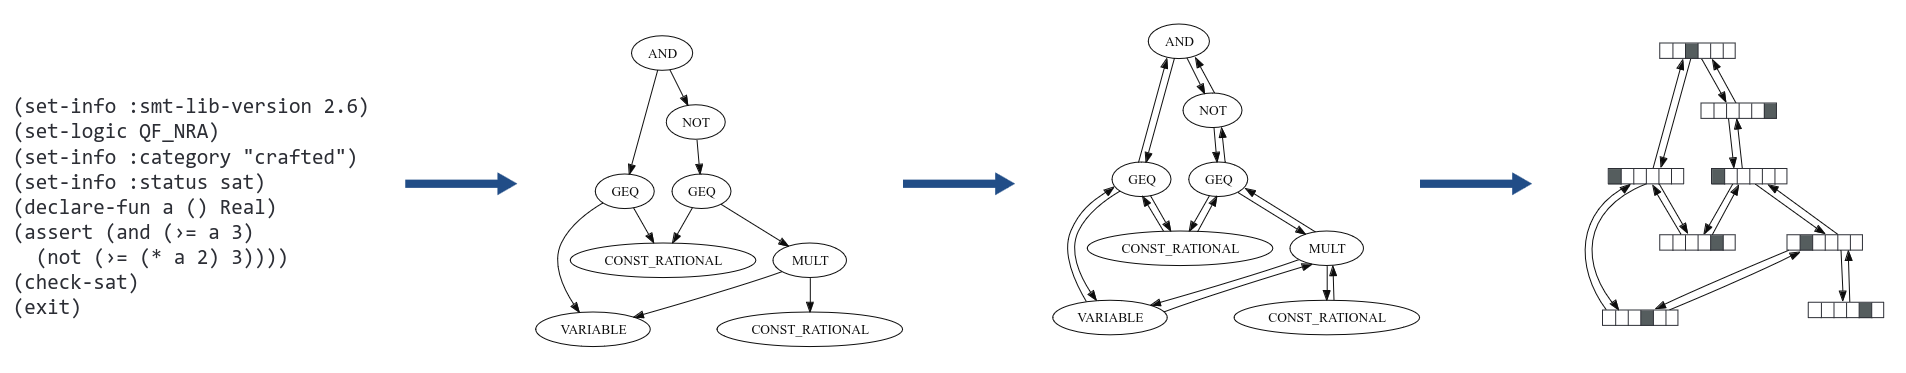
\includegraphics[scale=0.24]{./assets/gnn-for-scheduling-architecture.png}
    \caption{\label{gnn-for-scheduling-architecture} Использование AST формулы в качестве графа вычислений для GNN. Картинка взята из статьи \cite{gnn-for-scheduling-paper}.}
\end{center}
\end{figure}

Чтобы ускорить работу, вершины дерева, отвечающие за эквивалентные выражения, склеиваются в одну, так что формула, на самом деле, превращается в ориентированный ациклический граф. Помимо этого, чтобы расширить распространение эмбеддинга с информацией, сохранённой в каждой вершине, к каждому ребру такого графа добавляется обратное ребро. Таким образом, информация начинает распространяться сразу во всех направлениях.

\begin{figure}[ht]
\begin{center}
    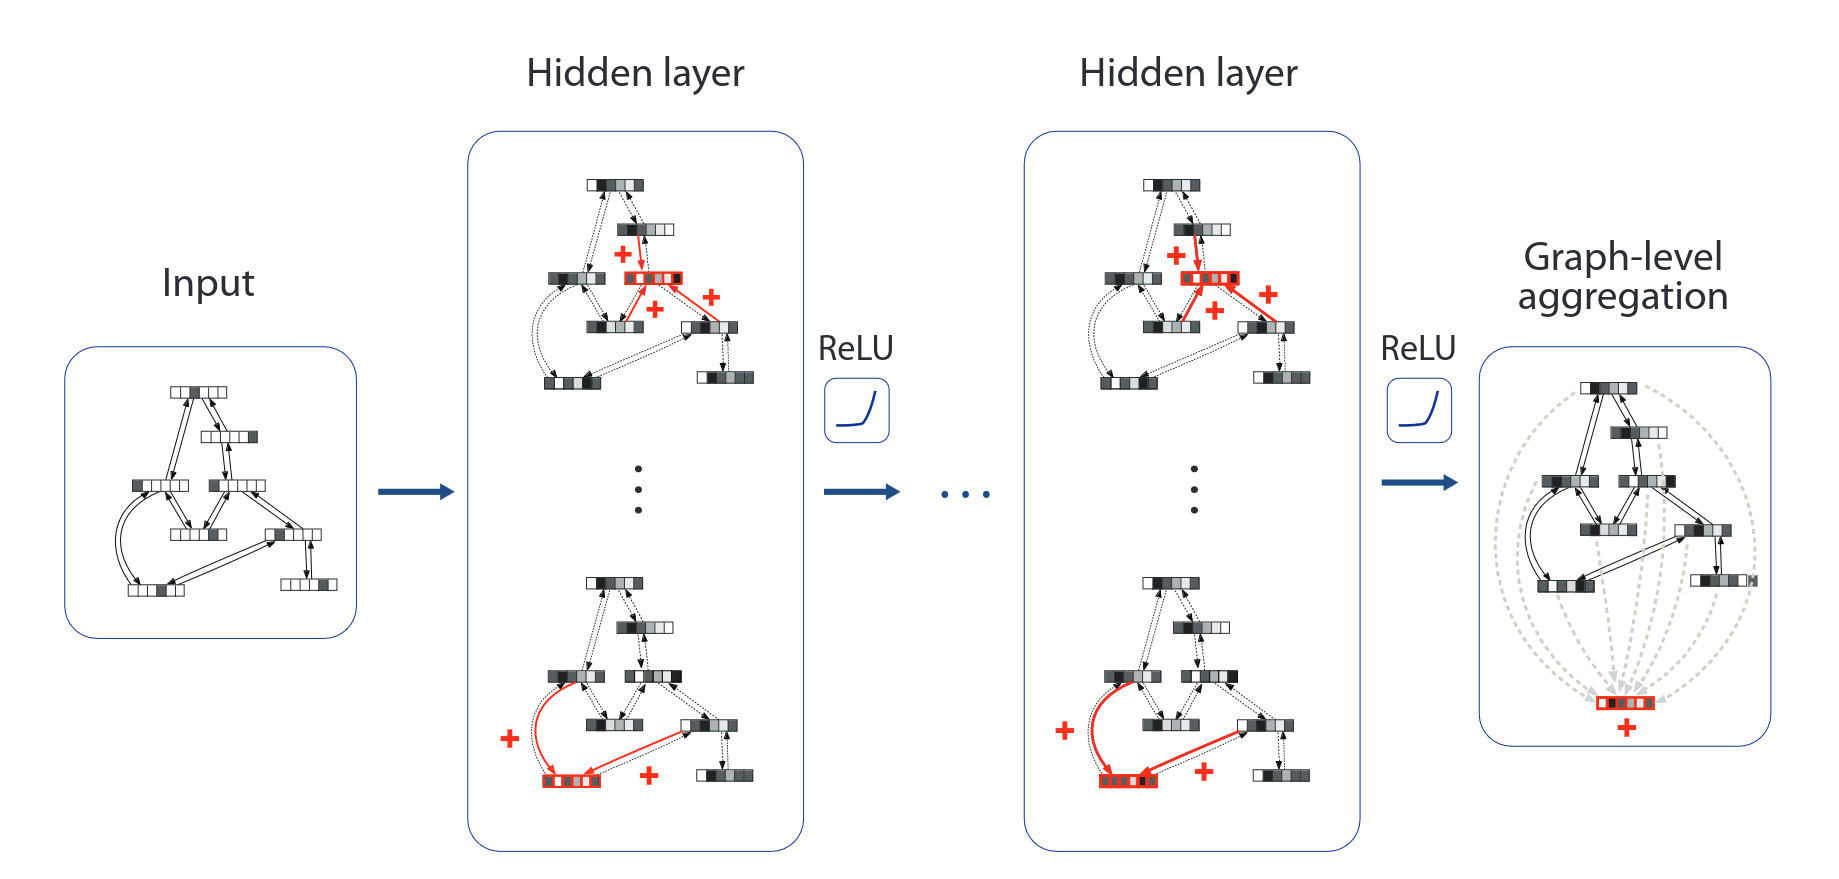
\includegraphics[scale=0.25]{./assets/gnn-for-scheduling-process.png}
    \caption{\label{gnn-for-scheduling-process} Схема использования GNN для получения информации о формуле и предсказания ответа. Картинка взята из статьи \cite{gnn-for-scheduling-paper}.}
\end{center}
\end{figure}

Далее каждая вершина (переменная, константа или операция) кодируется с помощью техники one-hot-encoding, после чего векторы с полученными таким образом значениями отправляются в GNN, на выходе у которой находится слой, собирающий эмбеддинги со всех вершин графа и предсказывающий для каждого SMT-решателя время, за которое он может выдать ответ на данной формуле. Для лучшего понимания, схема процесса изображена на рис~\ref{gnn-for-scheduling-process}.

Авторы отмечают, что подход может быть применён для решения почти для любой SMT-формулы, и утверждают, что им удалось добиться ускорения процесса на 8--900\% на разных тестах.

\specialsubsection{NeuroSAT}

Тем не менее, попытки научиться решать формально-логическую задачу, пользуясь исключительно нейронными сетями, тоже присутствуют. Пионером в этой области стала работа \cite{neurosat-paper}, в которой исследовалось применение GNN для задачи SAT. Была предложена следующая графовая архитектура: для каждой переменной, для отрицания каждой переменной и для каждого конъюнкта формулы заводится по вершине; далее рёбра проводятся между парами из литерала (переменными или их отрицаниями) и конъюнкта, если литерал входит в состав конъюнкта, а также между парами противоположных литералов (теми, которые является отрицаниями друг друга). Пример построения такого графа изображён на рис.~\ref{neurosat-mpnn}.

\begin{figure}[ht]
\begin{center}
    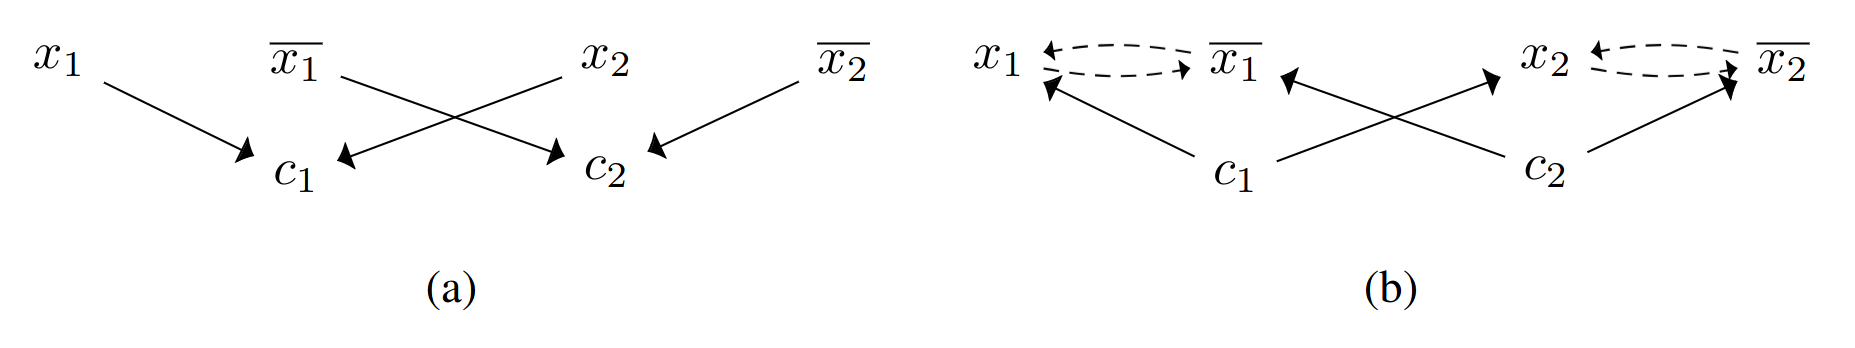
\includegraphics[scale=0.25]{./assets/neurosat-mpnn.png}
    \caption{\label{neurosat-mpnn} Граф, построенный для формулы $(x_1 \vee x_2) \wedge (\overline{x_1} \vee \overline{x_2})$. Пункты (a) и (b) отражают шаги построения, описанные в статье; на деле же граф выглядит как их объединение. Картинка взята из статьи \cite{neurosat-paper}.}
\end{center}
\end{figure}

Во время вычислений каждая вершина накапливает все пришедшие к ней сообщения с помощью LSTM-слоя. После каждого шага передачи сообщений по графу каждая вершина-литерал генерирует собственное предсказание по поводу того, является ли данная формула выполнимой (внутреннее состояние LSTM отправляется в многослойный классификатор (MLP), который предсказывает одно число --- степень уверенности вершины в том, что формула выполнима).

\begin{figure}[ht]
\begin{center}
    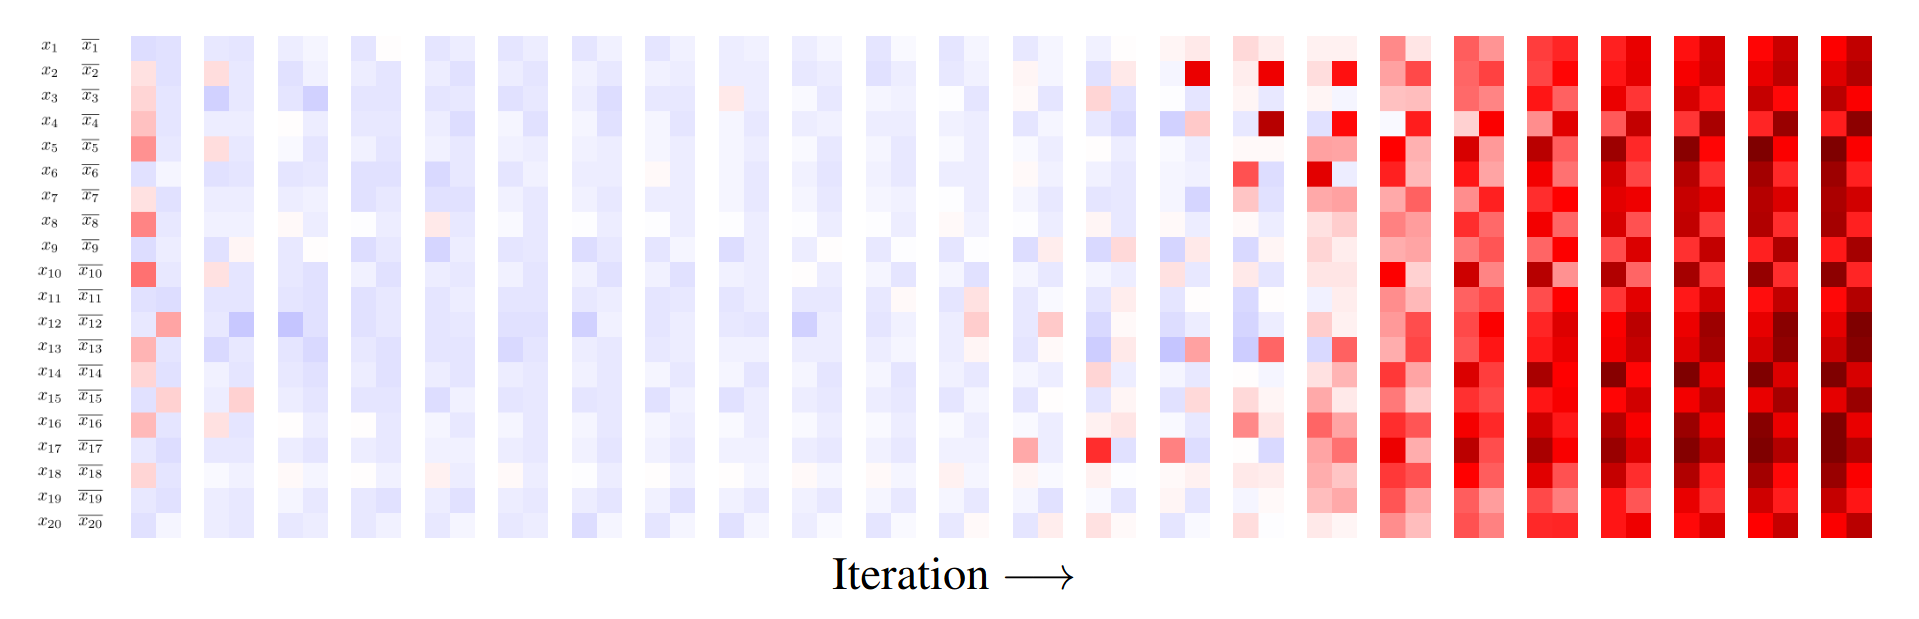
\includegraphics[scale=0.24]{./assets/neurosat-voting.png}
    \caption{\label{neurosat-voting} Граф, построенный для формулы $(x_1 \vee x_2) \wedge (\overline{x_1} \vee \overline{x_2})$. Пункты (a) и (b) отражают шаги построения, описанные в статье; на деле же граф выглядит как их объединение. Картинка взята из статьи \cite{neurosat-paper}.}
\end{center}
\end{figure}

% эмбеддинги
% дописать про GatedGraphConv https://pytorch-geometric.readthedocs.io/en/latest/generated/torch_geometric.nn.conv.GatedGraphConv.html#torch_geometric.nn.conv.GatedGraphConv
% слой голосования
% итерации
% результаты
% случайные формулы

% \hrule

% todo: дописать про другие работы
% \specialsubsection{Другие работы}

% mach smt
% alpha geometry
% Learning the Satisfiability of Pseudo-Boolean Problem with Graph Neural Networks
% https://ruoyuwang.me/bar2019/pdfs/bar2019-final80.pdf
% https://www.semanticscholar.org/paper/Algorithm-selection-for-SMT-Scott-Niemetz/aff1afe03f8e2f636b972add9b03ac59f6c34223
% https://www.semanticscholar.org/paper/On-EDA-Driven-Learning-for-SAT-Solving-Li-Shi/5c4bb681fe5cb159b0d577b784fa52c952871e17
% https://www.semanticscholar.org/paper/SATformer%3A-Transformer-Based-UNSAT-Core-Learning-Shi-Li/06547a615390ba14d37c684136c30a4ac559d610
% https://www.semanticscholar.org/paper/NeuroBack%3A-Improving-CDCL-SAT-Solving-using-Graph-Wang-Hu/a613142147ef740b2daf1265e23606c80d1c2bd2
% https://www.semanticscholar.org/paper/Synthesizing-Smart-Solving-Strategy-for-Symbolic-Chen-Chen/c7f8cd87ae269bb8b85eeb627005b7884a81bee0
% Combinatorial Optimization with Graph Convolutional Networks and Guided Tree Search https://arxiv.org/abs/1810.10659
% Andrew W Senior, Richard Evans, John Jumper, James Kirkpatrick, Laurent Sifre, Tim Green, Chongli Qin, Augustin Žídek, Alexander WR Nelson, Alex Bridgland, et al. Improved protein structure prediction using potentials from deep learning. Nature, 577(7792):706–710, 2020.